\documentclass{article}
\usepackage[preprint]{neurips_2021}
\usepackage[T1]{fontenc}
\usepackage[utf8]{inputenc}
\usepackage{graphicx}
\usepackage{booktabs}
\usepackage{caption}
\usepackage{subcaption}
\usepackage{enumitem}
\usepackage{adjustbox}

\title{Temporary Figure Gallery for CDA Paper Planning}
\author{}
\date{}

\begin{document}
\maketitle

\begin{center}
\fbox{%
\begin{minipage}{0.93\linewidth}
\small
\textbf{Important.} Every figure in this document uses \emph{synthetic illustrative values} created only to preview layout, visual style, and narrative structure. These are not real experimental claims and should not be copied into the paper as results.
\end{minipage}}
\end{center}

\section*{Goal}
This temporary document previews what the empirical and diagnostic figure program could look like if the paper presents a broad domain-generalization story against common baselines such as ERM, SWAD, and DIWA while emphasizing the CDA-based method family.

\section*{Main-Paper Candidates}

\begin{figure}[p]
    \centering
    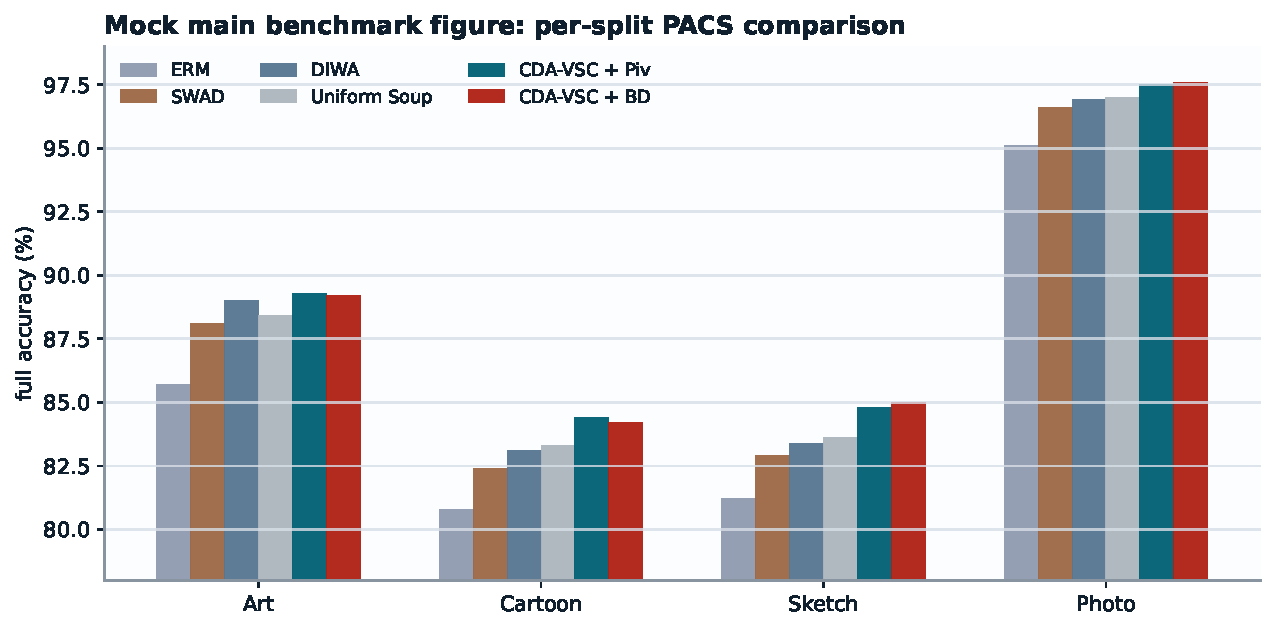
\includegraphics[width=\linewidth]{figures_mockups/01_main_benchmark.pdf}
    \caption{\textbf{Mock main benchmark comparison.} Grouped bars compare ERM, SWAD, DIWA, a uniform soup baseline, and the two CDA variants on each PACS target split. This is the most conventional ``main result'' figure and gives the reader an immediate sense of split-wise behavior and whether the proposed method is consistently competitive.}
\end{figure}
\clearpage

\begin{figure}[p]
    \centering
    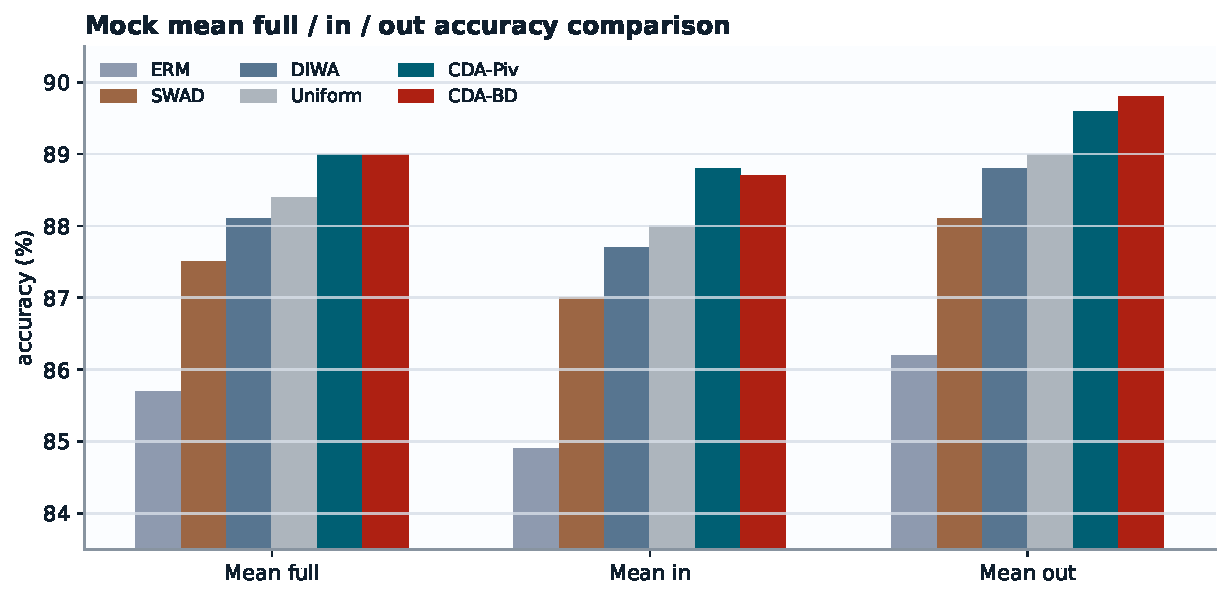
\includegraphics[width=\linewidth]{figures_mockups/02_mean_metrics.pdf}
    \caption{\textbf{Mock average full / in / out accuracy figure.} This figure would pair naturally with a table in the paper and makes it easy to show whether a method improves only pooled accuracy or also improves the out partition that is most relevant to the CDA narrative.}
\end{figure}
\clearpage

\begin{figure}[p]
    \centering
    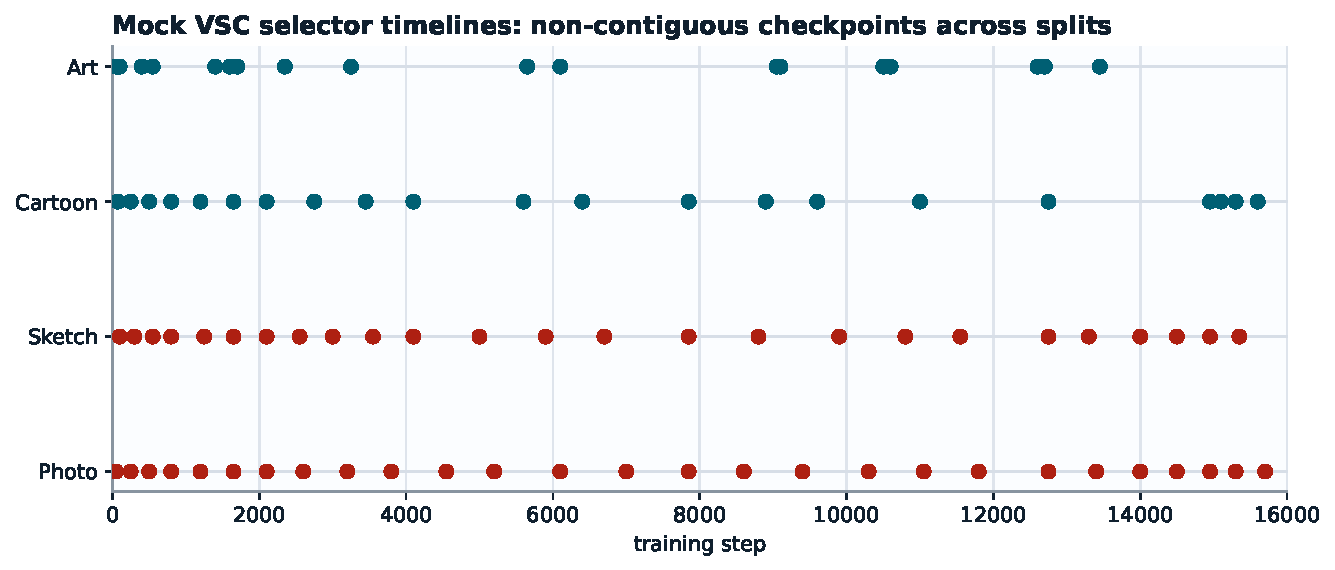
\includegraphics[width=\linewidth]{figures_mockups/03_checkpoint_timeline.pdf}
    \caption{\textbf{Mock non-contiguous checkpoint timeline.} Each row shows the retained checkpoints on one target split. This figure is designed to support the claim that the selected family need not be a contiguous late-training window in order to be averageable and useful.}
\end{figure}
\clearpage

\begin{figure}[p]
    \centering
    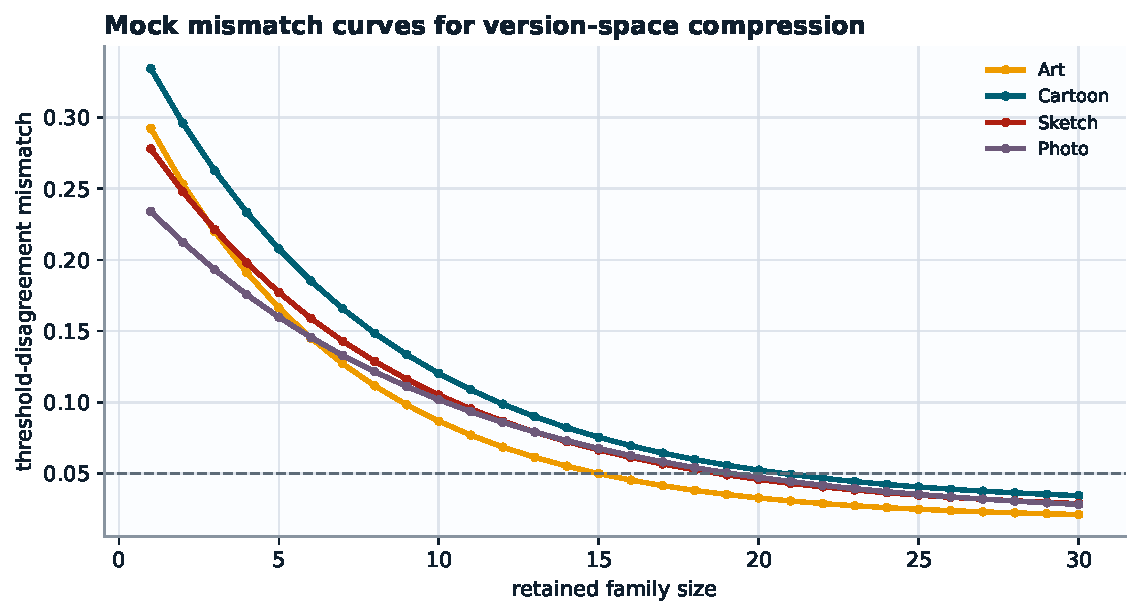
\includegraphics[width=\linewidth]{figures_mockups/04_vsc_mismatch.pdf}
    \caption{\textbf{Mock VSC mismatch curves.} The horizontal axis is retained family size and the vertical axis is disagreement mismatch to the full checkpoint bank. This is the cleanest selector-specific diagnostic because it shows whether added checkpoints are genuinely preserving the bank's source-support structure rather than merely increasing size.}
\end{figure}
\clearpage

\begin{figure}[p]
    \centering
    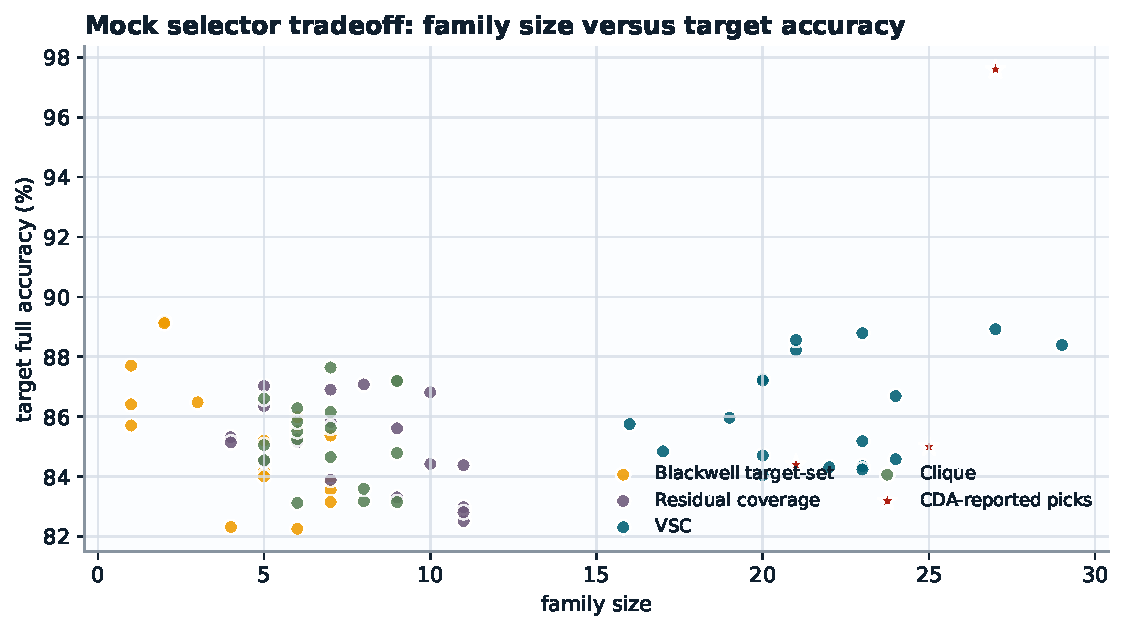
\includegraphics[width=\linewidth]{figures_mockups/05_family_size_vs_accuracy.pdf}
    \caption{\textbf{Mock selector tradeoff plot.} Each point is a selector instance; the horizontal axis is family size and the vertical axis is target accuracy. This figure is useful for showing that over-compression to tiny families can kill the weighting story even when a selector looks strong on a single split.}
\end{figure}
\clearpage

\begin{figure}[p]
    \centering
    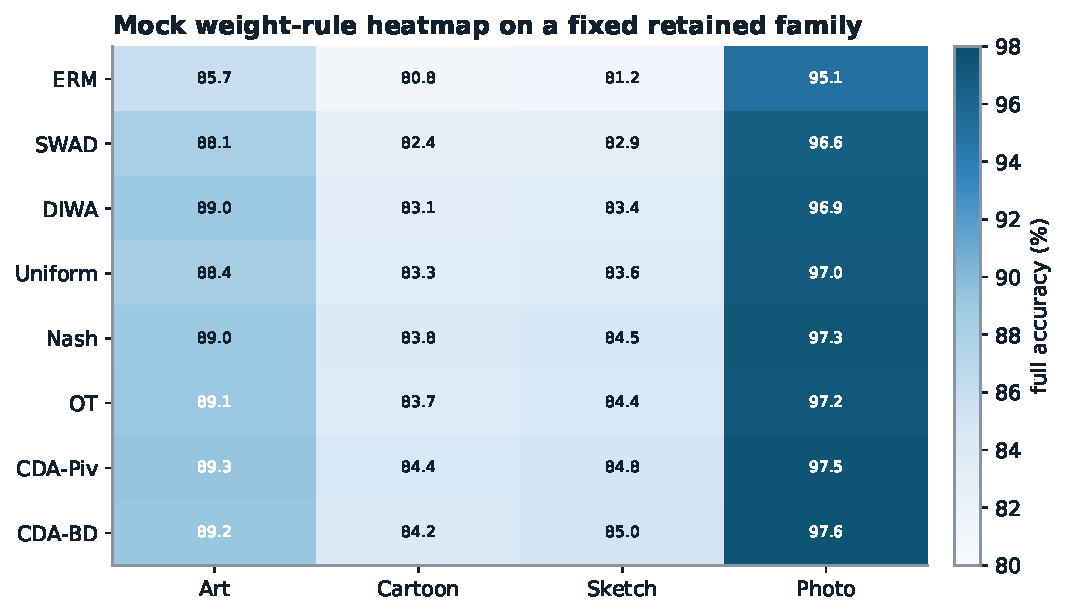
\includegraphics[width=\linewidth]{figures_mockups/06_weight_heatmap.pdf}
    \caption{\textbf{Mock fixed-selector heatmap over weight rules.} The heatmap visualizes how different weighting rules behave once the selector is frozen. This figure helps distinguish whether the observed gains are uniquely tied to the proposed CDA-derived rules or whether several weighting strategies occupy the same performance band.}
\end{figure}
\clearpage

\begin{figure}[p]
    \centering
    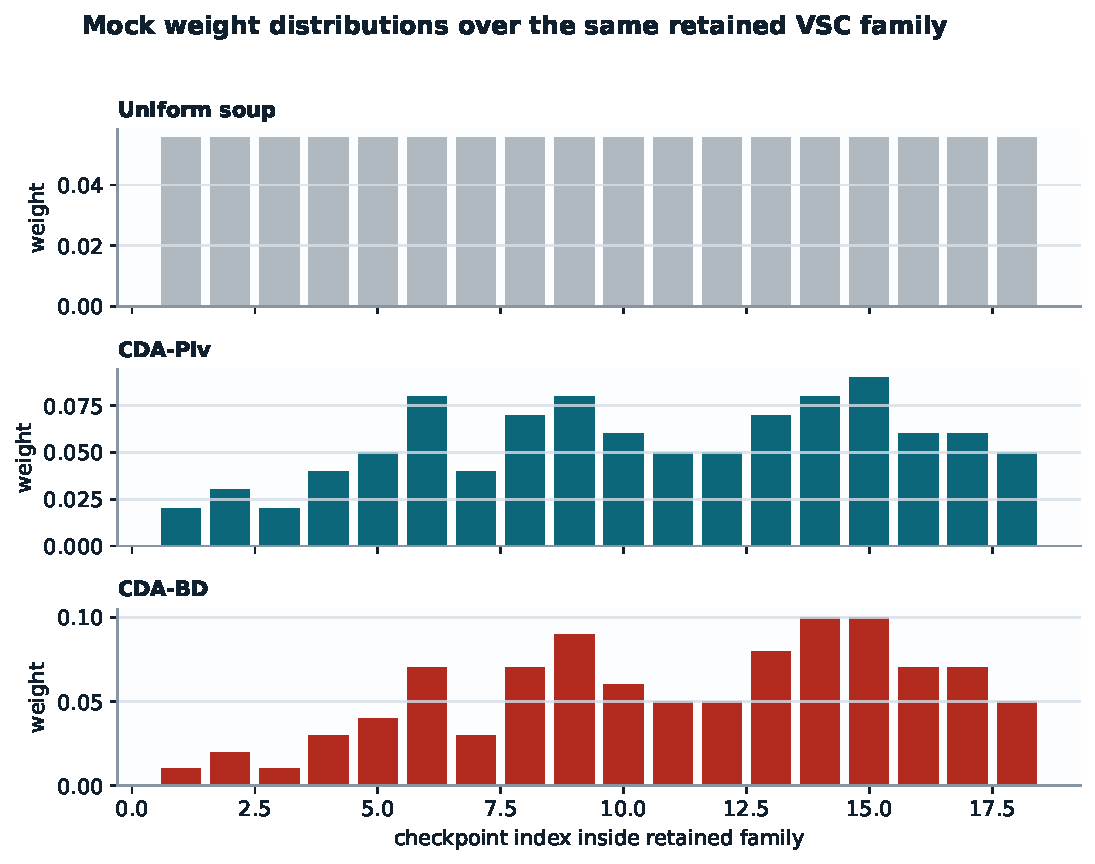
\includegraphics[width=\linewidth]{figures_mockups/07_weight_distribution.pdf}
    \caption{\textbf{Mock weight profiles on the same retained family.} The three panels compare uniform weighting, the pivotality-based rule, and the Blackwell-dual rule on the same checkpoint family. This is one of the most concrete ways to show that the proposed methods are not black boxes: they visibly reshape mass over the family rather than simply returning something uniform.}
\end{figure}
\clearpage

\begin{figure}[p]
    \centering
    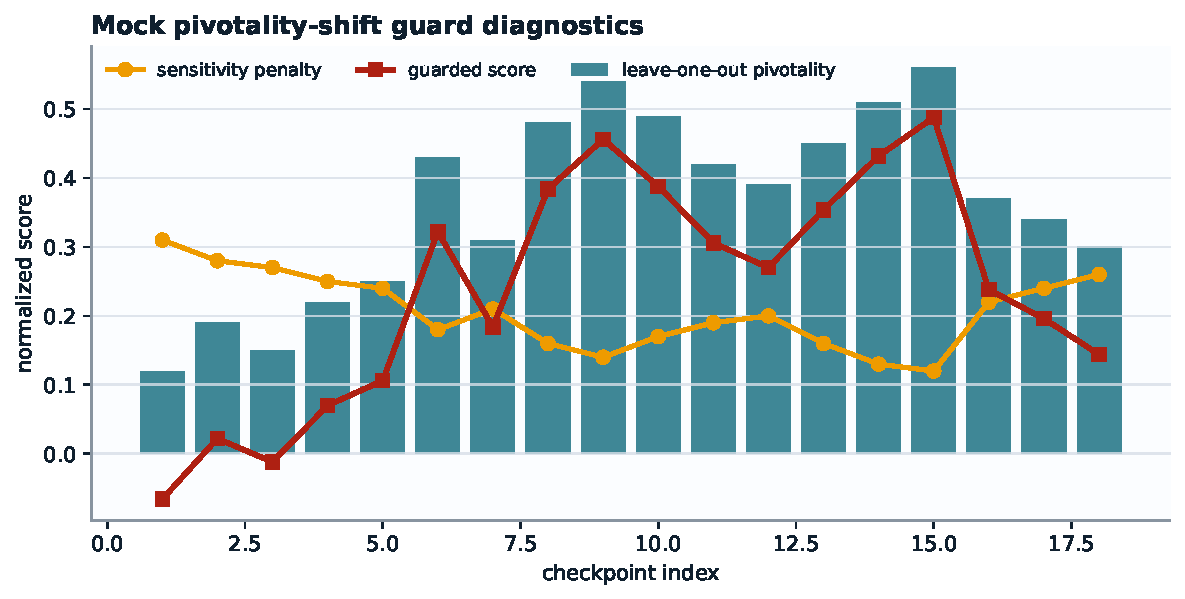
\includegraphics[width=\linewidth]{figures_mockups/08_pivotality_guard.pdf}
    \caption{\textbf{Mock pivotality-shift guard diagnostics.} Bars show leave-one-out pivotality, the line shows the sensitivity penalty, and the final guarded score is overlaid. This figure would make the \texttt{pivotality\_shift\_guard} mechanism much easier for readers to understand than equations alone.}
\end{figure}
\clearpage

\begin{figure}[p]
    \centering
    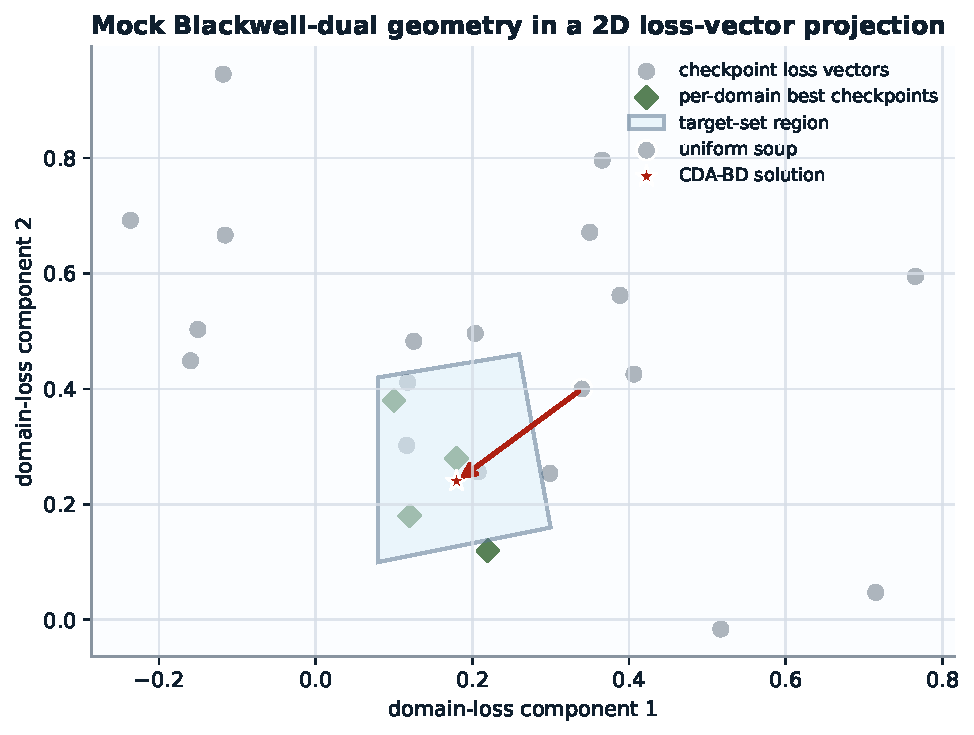
\includegraphics[width=\linewidth]{figures_mockups/09_blackwell_geometry.pdf}
    \caption{\textbf{Mock Blackwell-dual geometry.} Checkpoint domain-loss vectors are shown in a low-dimensional projection, together with a target-set region and the movement from a uniform soup toward the Blackwell-dual solution. This is the most intuitive empirical figure for the geometry of the dual weighting rule.}
\end{figure}
\clearpage

\begin{figure}[p]
    \centering
    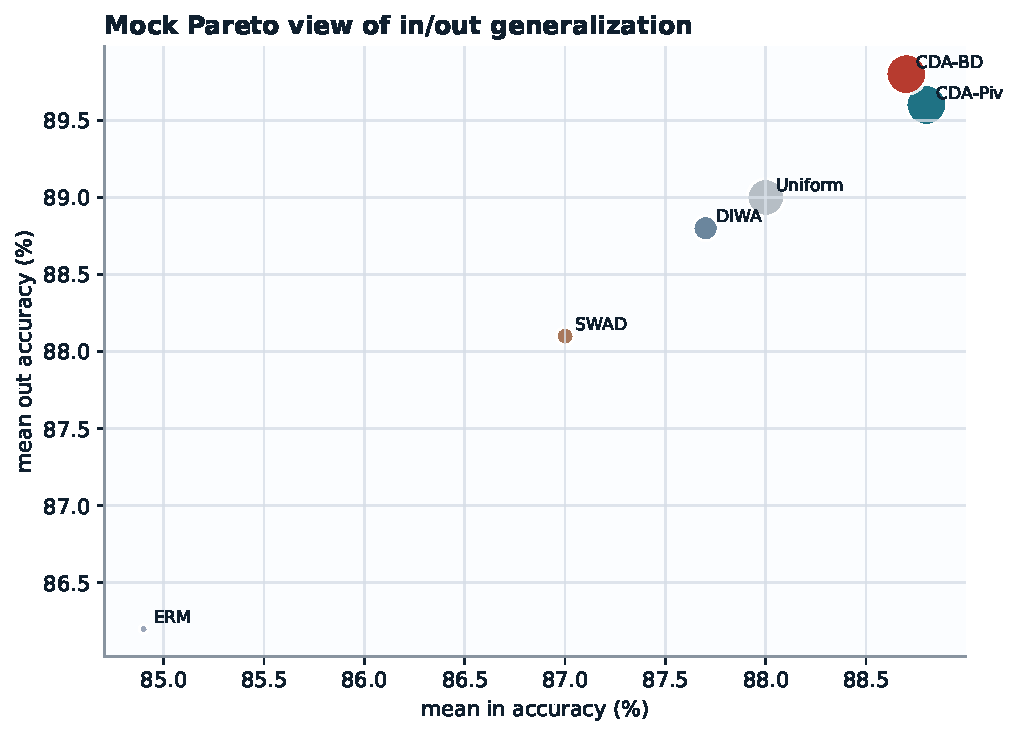
\includegraphics[width=\linewidth]{figures_mockups/10_pareto_in_out.pdf}
    \caption{\textbf{Mock in-vs-out Pareto plot.} Each method is shown as a point in the in/out plane, with point size representing retained-family scale. This figure is useful when the paper wants to show that a method is not winning only by sacrificing one partition for the other.}
\end{figure}
\clearpage

\section*{Theory-to-Empirics Bridge Figures}

\begin{figure}[p]
    \centering
    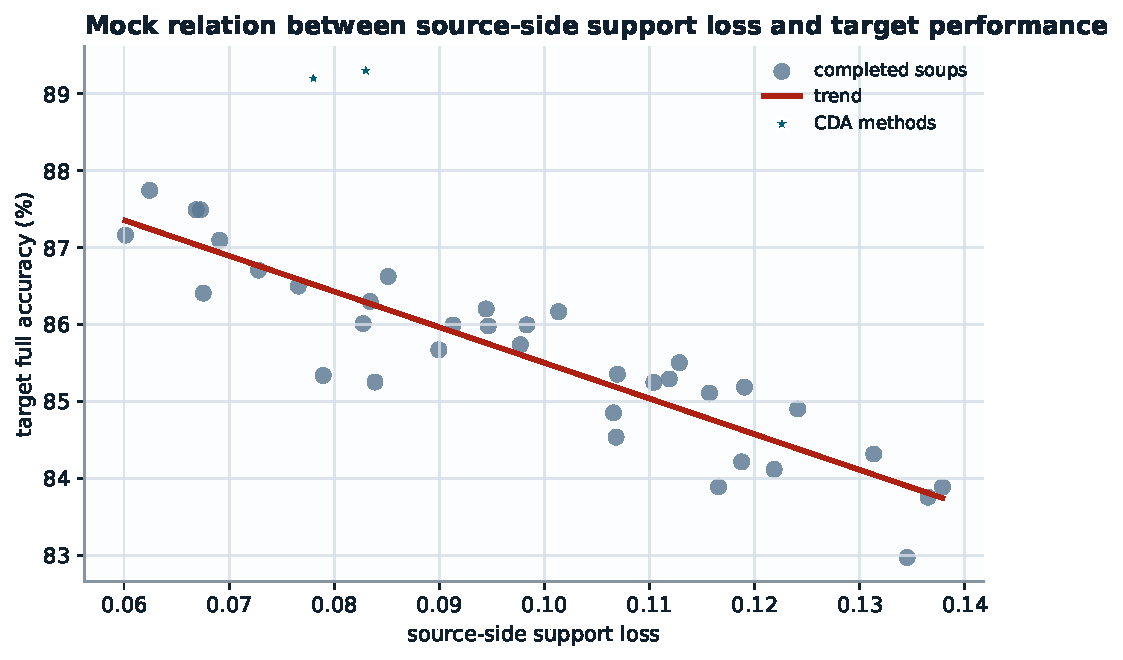
\includegraphics[width=\linewidth]{figures_mockups/11_support_vs_target.pdf}
    \caption{\textbf{Mock source-side proxy versus target accuracy.} This plot is designed to test whether a source-only diagnostic such as support loss or a CDA proxy actually predicts target behavior. If the paper wants its theory to do explanatory work, a figure of this kind is important.}
\end{figure}
\clearpage

\begin{figure}[p]
    \centering
    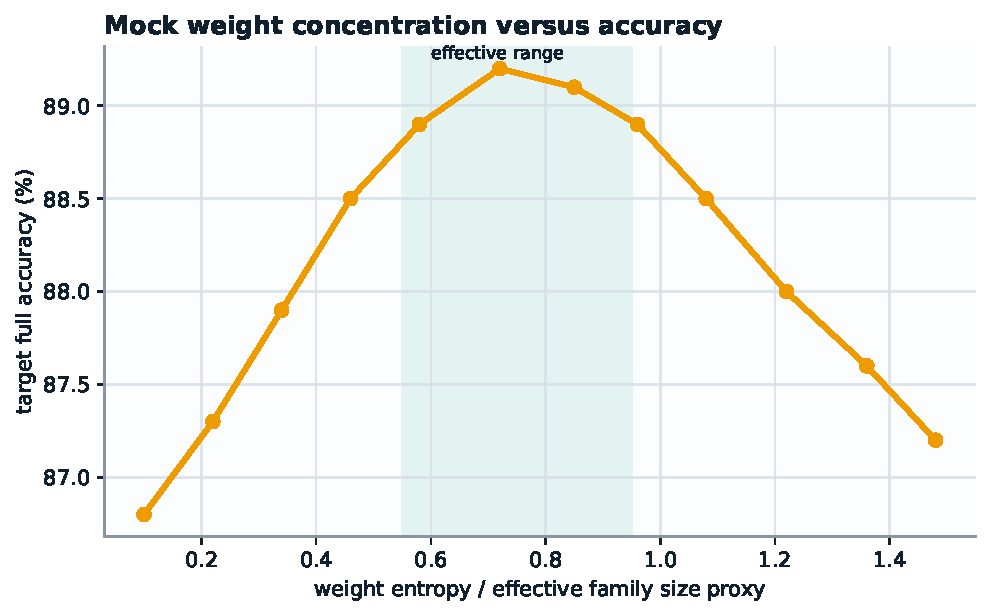
\includegraphics[width=\linewidth]{figures_mockups/12_entropy_vs_accuracy.pdf}
    \caption{\textbf{Mock weight concentration versus accuracy.} The horizontal axis reflects how concentrated the final weights are. This helps show whether the method improves by learning a meaningful mixture or by collapsing onto a near-singleton solution.}
\end{figure}
\clearpage

\begin{figure}[p]
    \centering
    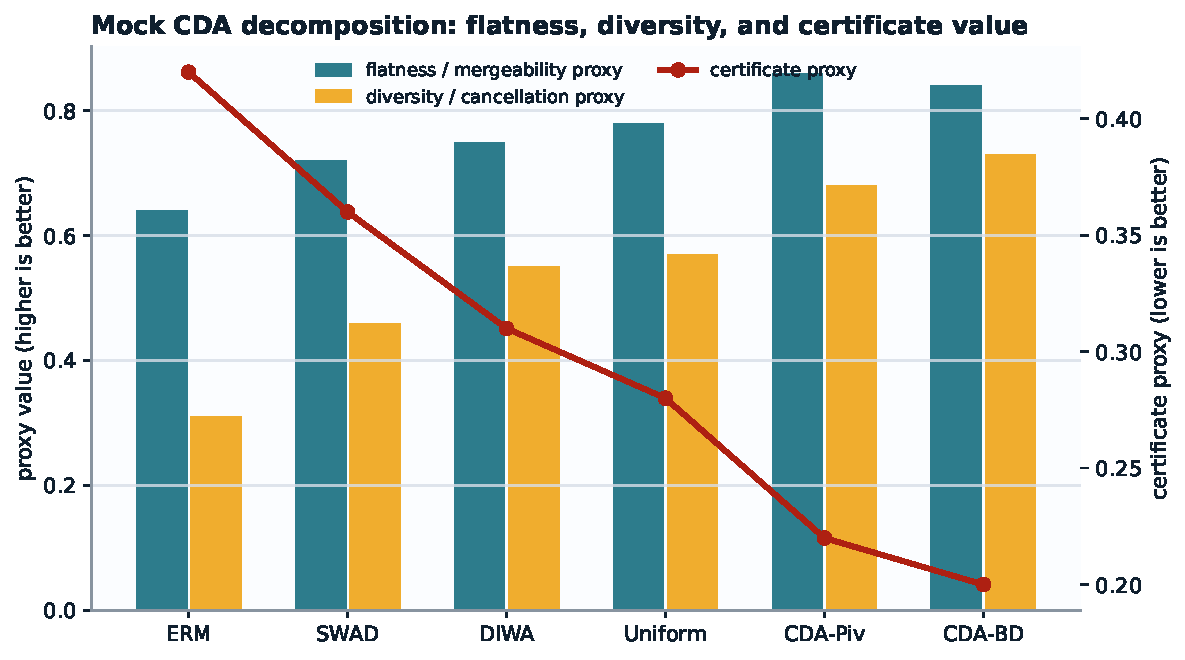
\includegraphics[width=\linewidth]{figures_mockups/13_certificate_components.pdf}
    \caption{\textbf{Mock CDA decomposition plot.} The bars represent flatness / mergeability and diversity / cancellation proxies, while the line shows a certificate proxy. This figure would visually support the unifying claim that apparently different successful heuristics are reducing different parts of the same source-side criterion.}
\end{figure}
\clearpage

\begin{figure}[p]
    \centering
    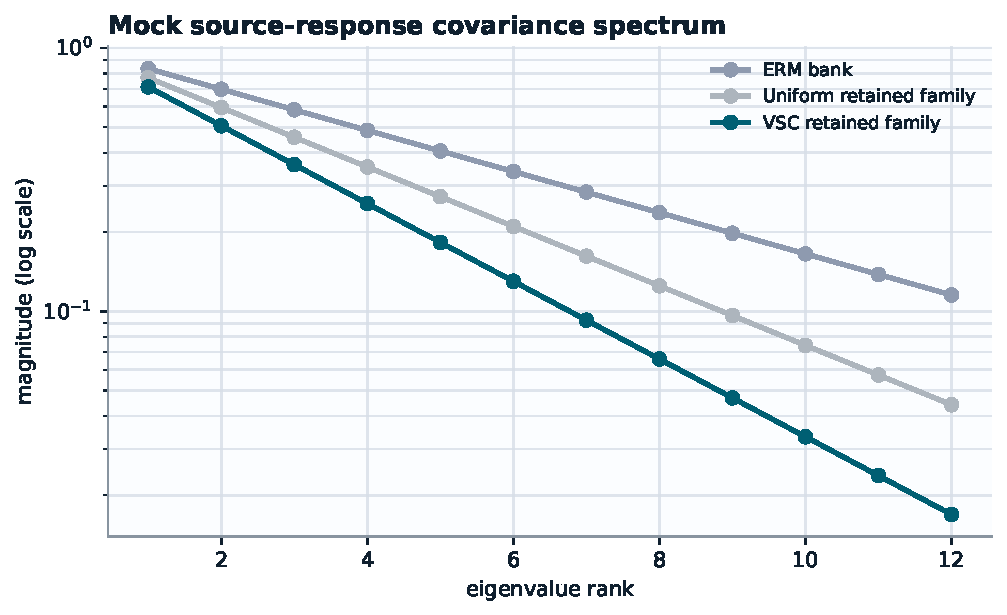
\includegraphics[width=\linewidth]{figures_mockups/14_covariance_spectrum.pdf}
    \caption{\textbf{Mock covariance spectrum diagnostic.} This scree-style figure shows how much domain-response variation remains after family compression. It is a natural visual for the claim that version-space compression preserves the important low-dimensional disagreement geometry of the full bank.}
\end{figure}
\clearpage

\begin{figure}[p]
    \centering
    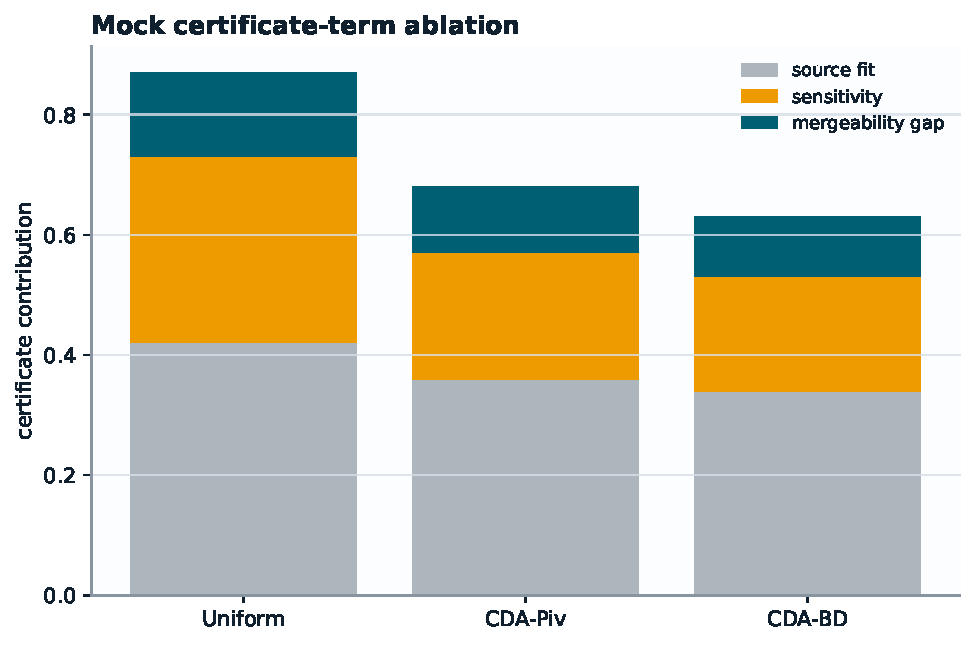
\includegraphics[width=\linewidth]{figures_mockups/15_certificate_ablation.pdf}
    \caption{\textbf{Mock certificate-term ablation.} Each stacked bar decomposes a source-supported certificate into source fit, mixture sensitivity, and mergeability gap. This is a strong figure if the paper wants to demonstrate that the proposed methods help for the reason the theory predicts, not just because they score well.}
\end{figure}
\clearpage

\section*{Appendix-Style Diagnostics}

\begin{figure}[p]
    \centering
    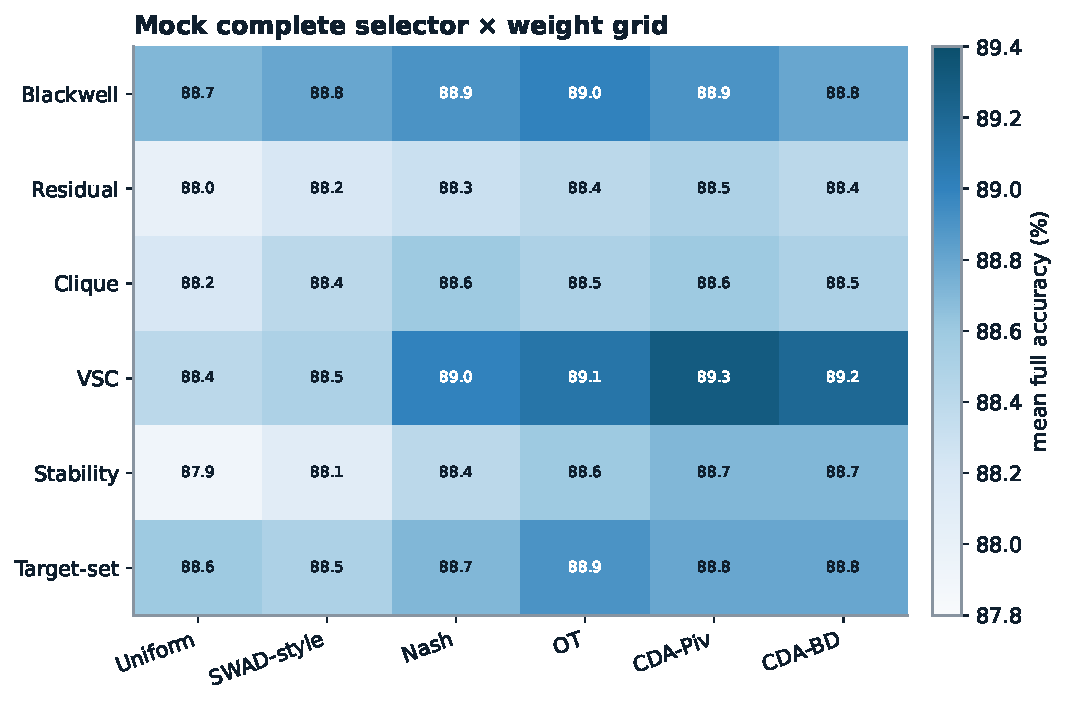
\includegraphics[width=\linewidth]{figures_mockups/16_full_cross_heatmap.pdf}
    \caption{\textbf{Mock full selector-by-weight heatmap.} This appendix-style figure visualizes the broader search space after the main method is chosen. It is useful for showing that the final method was selected from a landscape with meaningful structure rather than from a flat sea of near-identical results.}
\end{figure}
\clearpage

\begin{figure}[p]
    \centering
    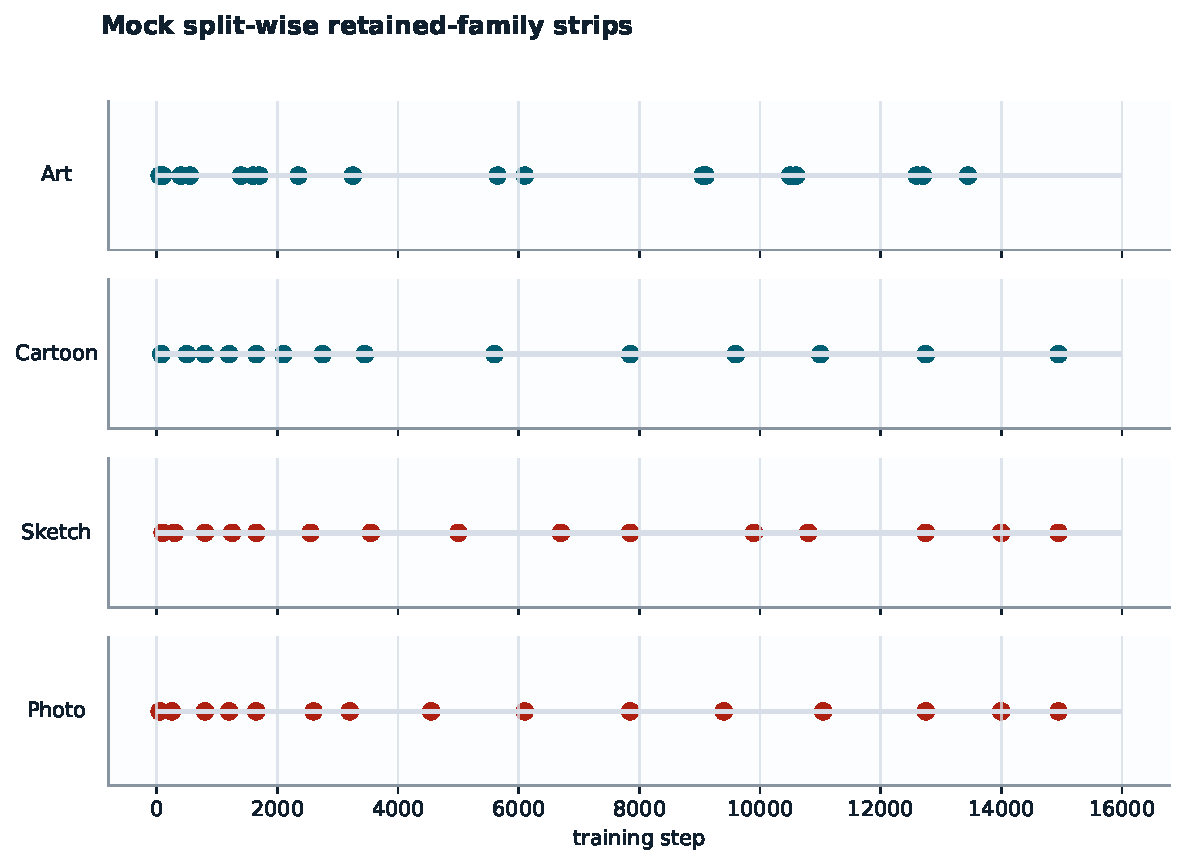
\includegraphics[width=\linewidth]{figures_mockups/17_family_strips.pdf}
    \caption{\textbf{Mock split-wise retained-family strips.} This is a compact appendix-friendly way to show exactly which checkpoints were retained on each split without forcing the reader to parse a long list of step indices in the main text.}
\end{figure}
\clearpage

\begin{figure}[p]
    \centering
    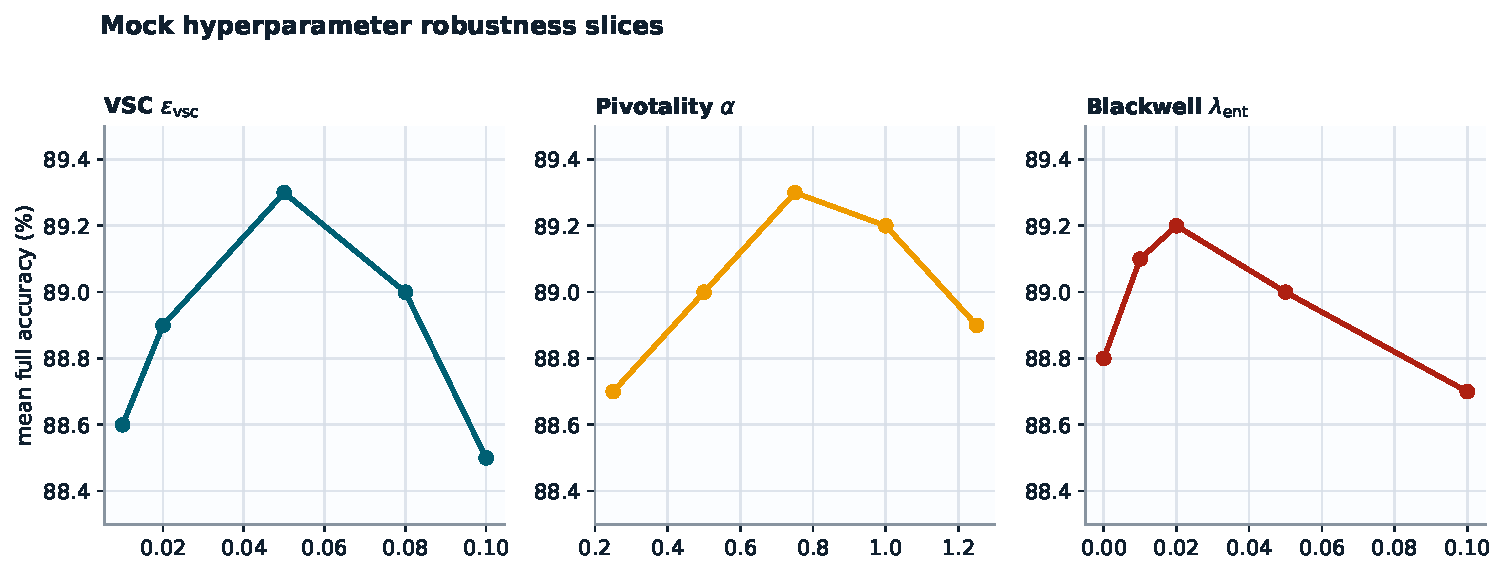
\includegraphics[width=\linewidth]{figures_mockups/18_hparam_robustness.pdf}
    \caption{\textbf{Mock hyperparameter robustness slices.} Each panel shows a one-dimensional slice through a selector or weighting-rule hyperparameter. This kind of figure helps distinguish a method that is scientifically stable from one that only works at a single lucky setting.}
\end{figure}
\clearpage

\begin{figure}[p]
    \centering
    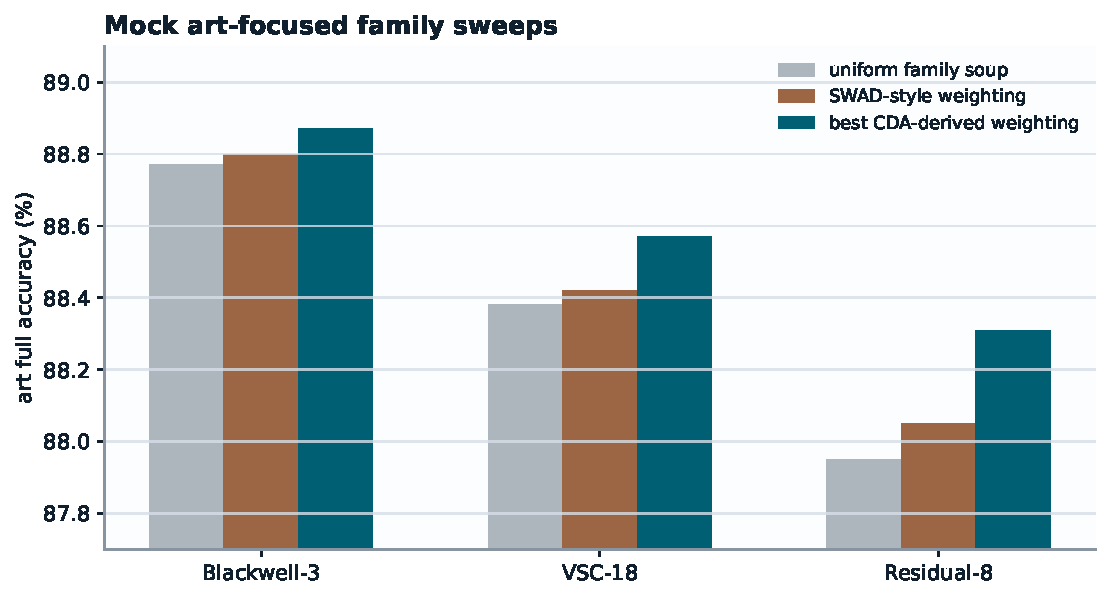
\includegraphics[width=\linewidth]{figures_mockups/19_art_family_sweeps.pdf}
    \caption{\textbf{Mock art-focused family sweeps.} This figure compares uniform family soups, SWAD-style weighting, and the best CDA-derived weighting across several art-focused families. It is a clean way to show that the benefit of nonuniform weighting depends on the geometry and size of the retained family.}
\end{figure}
\clearpage

\begin{figure}[p]
    \centering
    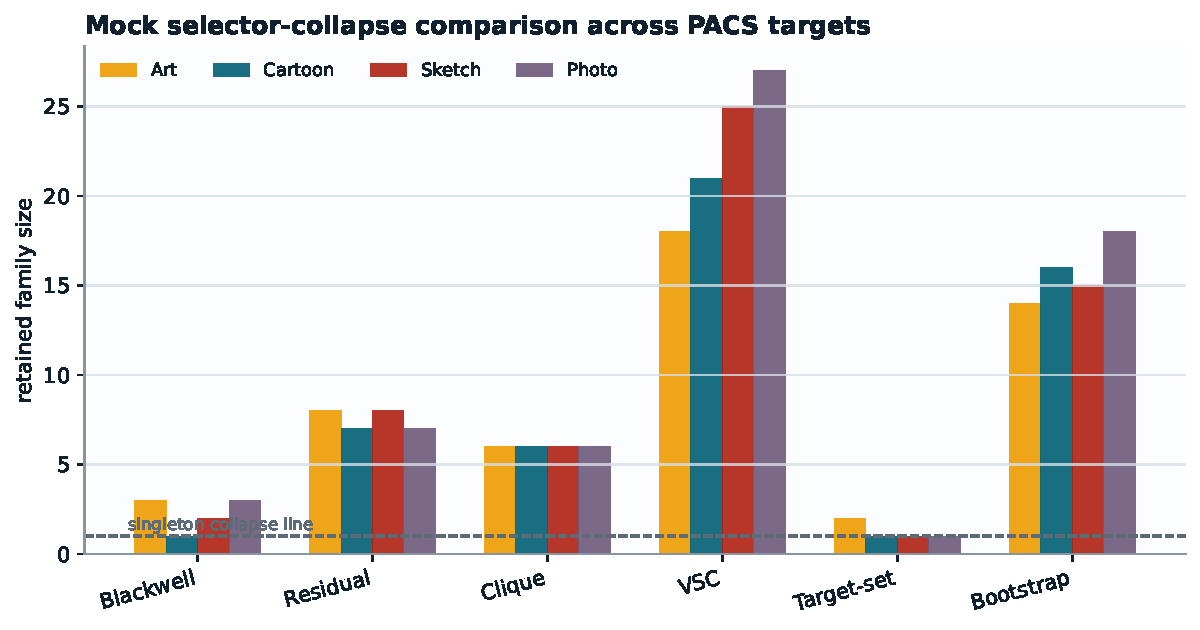
\includegraphics[width=\linewidth]{figures_mockups/20_selector_collapse.pdf}
    \caption{\textbf{Mock selector-collapse comparison.} Bars show retained family size across PACS target splits for several selector families. This figure directly supports the paper's argument that a selector can fail by collapsing too aggressively, even when it appears strong on one split.}
\end{figure}
\clearpage

\section*{How To Use This Preview}
\begin{itemize}[leftmargin=1.5em]
    \item Promote the strongest 6--8 figures into the main paper.
    \item Move the broader search-space plots into the appendix.
    \item Replace the synthetic numbers with real exports from the results ledger and replay artifacts once the final figure list is chosen.
\end{itemize}

\end{document}
